% Hình task/context từ EX01 đã lưu; không fit hoặc chạy inference nghiên cứu.
\documentclass[10pt]{article}
\usepackage[T1]{fontenc}
\usepackage{lmodern}
\usepackage[paperwidth=180mm,paperheight=185mm,margin=4mm]{geometry}
\usepackage{tikz}
\usetikzlibrary{arrows.meta}
\pagestyle{empty}
\setlength{\parindent}{0pt}
\hyphenpenalty=10000
\exhyphenpenalty=10000
\definecolor{ink}{HTML}{1F3445}
\definecolor{teal}{HTML}{126B80}
\definecolor{violet}{HTML}{6D548A}
\begin{document}
\centering
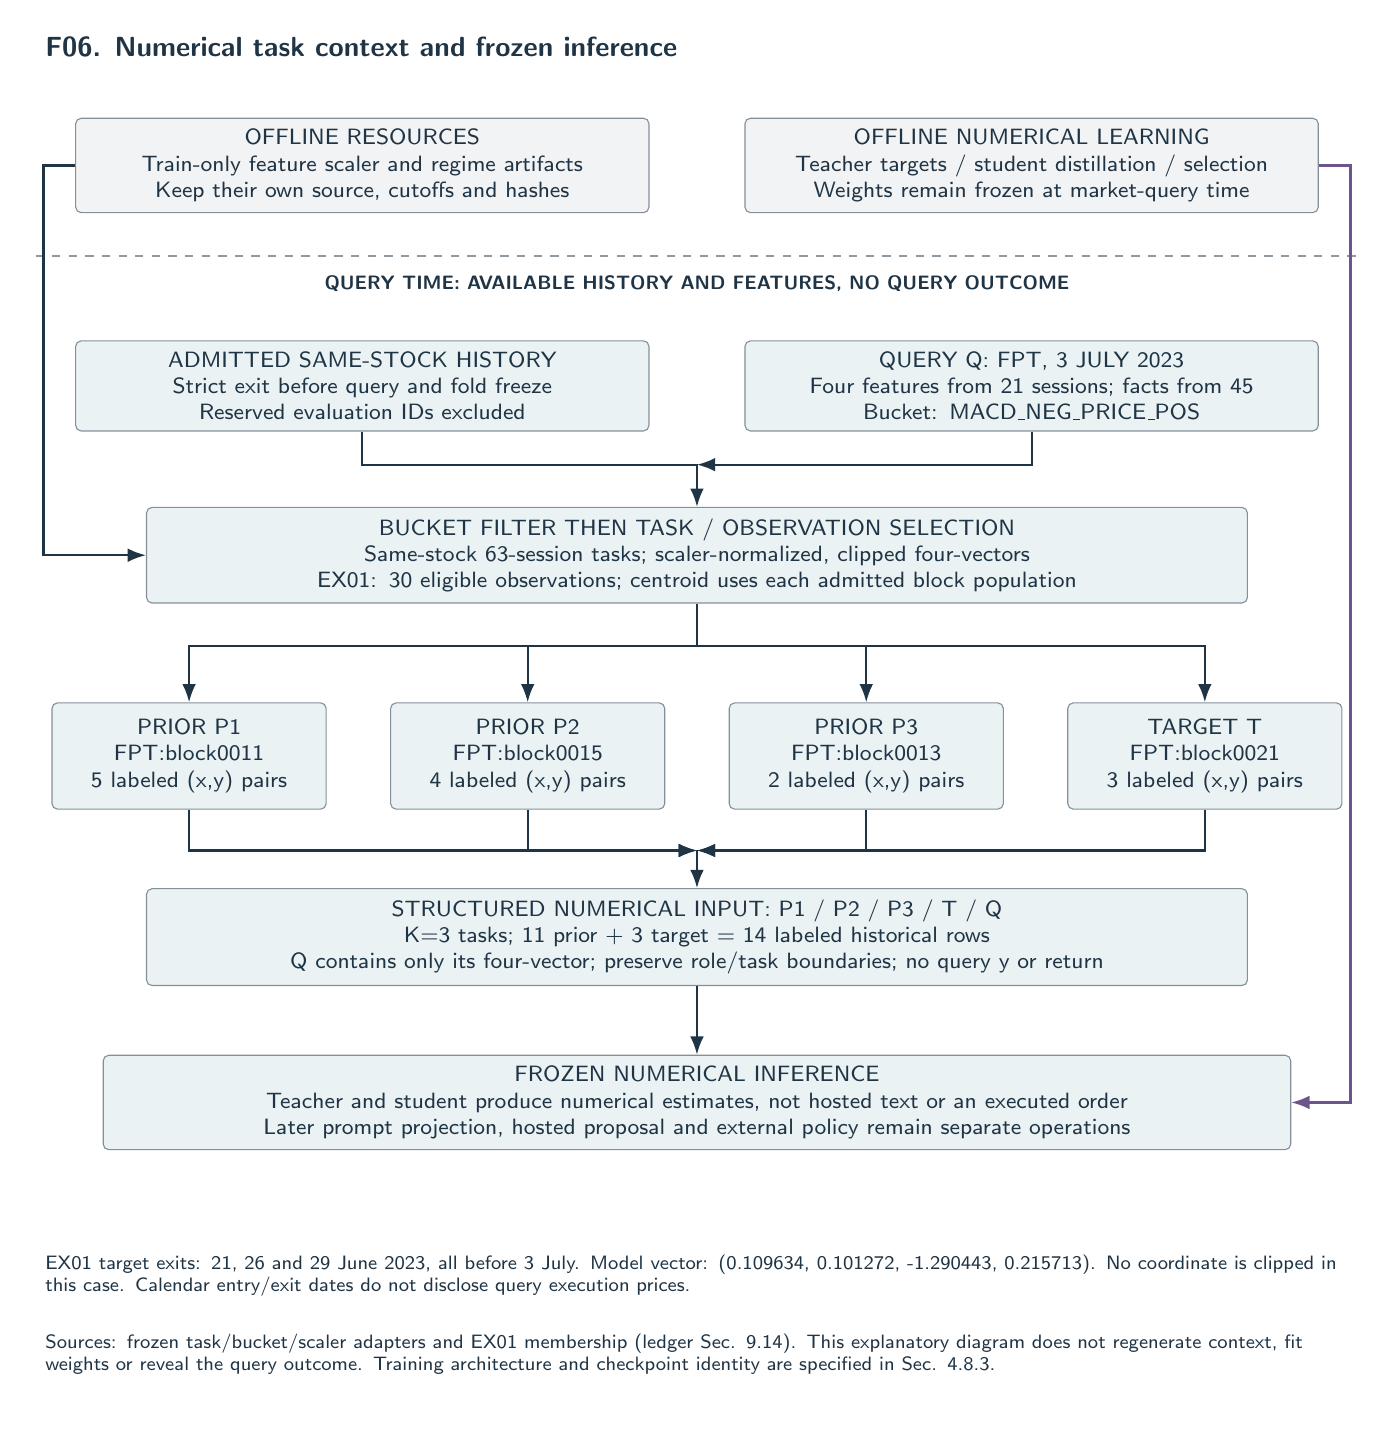
\begin{tikzpicture}[x=1cm,y=1cm,>=Latex,font=\sffamily\footnotesize,text=ink,
 box/.style={draw=ink!55,rounded corners=2pt,align=center,text width=7cm,minimum height=1.1cm,inner sep=4pt},
 flow/.style={->,thick,draw=ink}]
\path[use as bounding box] (0,0) rectangle (17.0,17.5);
\node[anchor=west,font=\sffamily\bfseries] at (.1,17.25) {F06. Numerical task context and frozen inference};
\node[box,fill=ink!6] (resources) at (4.25,15.75)
 {OFFLINE RESOURCES\\Train-only feature scaler and regime artifacts\\Keep their own source, cutoffs and hashes};
\node[box,fill=ink!6] (student) at (12.75,15.75)
 {OFFLINE NUMERICAL LEARNING\\Teacher targets / student distillation / selection\\Weights remain frozen at market-query time};
\draw[dashed,draw=ink!50] (.1,14.6) -- (16.9,14.6);
\node[font=\sffamily\bfseries\scriptsize] at (8.5,14.25)
 {QUERY TIME: AVAILABLE HISTORY AND FEATURES, NO QUERY OUTCOME};
\node[box,fill=teal!9] (history) at (4.25,12.95)
 {ADMITTED SAME-STOCK HISTORY\\Strict exit before query and fold freeze\\Reserved evaluation IDs excluded};
\node[box,fill=teal!9] (q) at (12.75,12.95)
 {QUERY Q: FPT, 3 JULY 2023\\Four features from 21 sessions; facts from 45\\Bucket: MACD\_NEG\_PRICE\_POS};
\node[box,fill=teal!9,text width=13.7cm] (selection) at (8.5,10.8)
 {BUCKET FILTER THEN TASK / OBSERVATION SELECTION\\Same-stock 63-session tasks; scaler-normalized, clipped four-vectors\\EX01: 30 eligible observations; centroid uses each admitted block population};
\draw[flow] (history.south) -- (4.25,11.95) -| (selection.north);
\draw[flow] (q.south) -- (12.75,11.95) -- (8.5,11.95);
\draw[flow] (resources.west) -- (.2,15.75) -- (.2,10.8) -- (selection.west);
\node[box,fill=teal!9,text width=3.2cm,minimum height=1.35cm] (p1) at (2.05,8.25)
 {PRIOR P1\\FPT:block0011\\5 labeled (x,y) pairs};
\node[box,fill=teal!9,text width=3.2cm,minimum height=1.35cm] (p2) at (6.35,8.25)
 {PRIOR P2\\FPT:block0015\\4 labeled (x,y) pairs};
\node[box,fill=teal!9,text width=3.2cm,minimum height=1.35cm] (p3) at (10.65,8.25)
 {PRIOR P3\\FPT:block0013\\2 labeled (x,y) pairs};
\node[box,fill=teal!9,text width=3.2cm,minimum height=1.35cm] (target) at (14.95,8.25)
 {TARGET T\\FPT:block0021\\3 labeled (x,y) pairs};
\draw[flow] (selection.south) -- (8.5,9.65) -| (p1.north);
\draw[flow] (8.5,9.65) -| (p2.north);
\draw[flow] (8.5,9.65) -| (p3.north);
\draw[flow] (8.5,9.65) -| (target.north);
\node[box,fill=teal!9,text width=13.7cm] (input) at (8.5,5.95)
 {STRUCTURED NUMERICAL INPUT: P1 / P2 / P3 / T / Q\\K=3 tasks; 11 prior + 3 target = 14 labeled historical rows\\Q contains only its four-vector; preserve role/task boundaries; no query y or return};
\foreach \source in {p1,p2,p3,target}
 {\draw[flow] (\source.south) -- (\source.south |- 8.5,7.05) -- (8.5,7.05);}
\draw[flow] (8.5,7.05) -- (input.north);
\node[box,fill=teal!9,text width=14.8cm] (inference) at (8.5,3.85)
 {FROZEN NUMERICAL INFERENCE\\Teacher and student produce numerical estimates, not hosted text or an executed order\\Later prompt projection, hosted proposal and external policy remain separate operations};
\draw[flow,draw=violet] (student.east) -- (16.8,15.75) -- (16.8,3.85) -- (inference.east);
\draw[flow] (input) -- (inference);
\node[anchor=west,align=left,text width=16.7cm,font=\sffamily\scriptsize] at (.1,1.65)
 {EX01 target exits: 21, 26 and 29 June 2023, all before 3 July. Model vector:
 (0.109634, 0.101272, -1.290443, 0.215713). No coordinate is clipped in this case.
 Calendar entry/exit dates do not disclose query execution prices.};
\node[anchor=west,align=left,text width=16.7cm,font=\sffamily\scriptsize] at (.1,.65)
 {Sources: frozen task/bucket/scaler adapters and EX01 membership (ledger Sec. 9.14).
 This explanatory diagram does not regenerate context, fit weights or reveal the query outcome.
 Training architecture and checkpoint identity are specified in Sec. 4.8.3.};
\end{tikzpicture}
\end{document}
